% File tacl2018v2.tex
% Sep 20, 2018

% The English content of this file was modified from various *ACL instructions
% by Lillian Lee and Kristina Toutanova
%
% LaTeXery is mostly all adapted from acl2018.sty.

\documentclass[11pt,a4paper]{article}
\usepackage{times,latexsym}
\usepackage{url}
\usepackage[T1]{fontenc}
\usepackage{graphicx}

%% Package options:
%% Short version: "hyperref" and "submission" are the defaults.
%% More verbose version:
%% Most compact command to produce a submission version with hyperref enabled
%%    \usepackage[]{tacl2018v2}
%% Most compact command to produce a "camera-ready" version
%%    \usepackage[acceptedWithA]{tacl2018v2}
%% Most compact command to produce a double-spaced copy-editor's version
%%    \usepackage[acceptedWithA,copyedit]{tacl2018v2}
%
%% If you need to disable hyperref in any of the above settings (see Section
%% "LaTeX files") in the TACL instructions), add ",nohyperref" in the square
%% brackets. (The comma is a delimiter in case there are multiple options specified.)

%\usepackage[]{tacl2018v2}
\usepackage[acceptedWithA]{tacl2018v2}

%%%% Material in this block is specific to generating TACL instructions
\usepackage{xspace,mfirstuc,tabulary}
\newcommand{\dateOfLastUpdate}{Sept. 20, 2018}
\newcommand{\styleFileVersion}{tacl2018v2}

\newcommand{\ex}[1]{{\sf #1}}

\newif\iftaclinstructions
\taclinstructionsfalse % AUTHORS: do NOT set this to true
\iftaclinstructions
\renewcommand{\confidential}{}
\renewcommand{\anonsubtext}{(No author info supplied here, for consistency with
TACL-submission anonymization requirements)}
\newcommand{\instr}
\fi

%
\iftaclpubformat % this "if" is set by the choice of options
\newcommand{\taclpaper}{final version\xspace}
\newcommand{\taclpapers}{final versions\xspace}
\newcommand{\Taclpaper}{Final version\xspace}
\newcommand{\Taclpapers}{Final versions\xspace}
\newcommand{\TaclPapers}{Final Versions\xspace}
\else
\newcommand{\taclpaper}{submission\xspace}
\newcommand{\taclpapers}{{\taclpaper}s\xspace}
\newcommand{\Taclpaper}{Submission\xspace}
\newcommand{\Taclpapers}{{\Taclpaper}s\xspace}
\newcommand{\TaclPapers}{Submissions\xspace}
\fi

%%%% End TACL-instructions-specific macro block
%%%%

% \title{Formatting Instructions for TACL \TaclPapers \\
% (Base files: \styleFileVersion-template.tex \& \styleFileVersion.sty, dated \dateOfLastUpdate)}
\title{Text classifications using IMapBook dataset}


% Author information does not appear in the pdf unless the "acceptedWithA" option is given
% See tacl2018v2.sty for other ways to format author information
\author{
 Domen Kos, Timotej Kovač \\
 University of Ljubljana \\
 Faculty of computer and information science \\
 Večna pot 113, SI-1000 Ljubljana \\
  {\sf dk6314@student.uni-lj.si, tk3713@student.uni-lj.si} \\
}

\date{}

\begin{document}
\maketitle
 \begin{abstract}
   TODO
 \end{abstract}


\section{Introduction}
For the course assignment at \textit{Natural language processing} class we decided to do text classification on IMapBook dataset.
The dataset contains short discussions between primary school students who are chatting about different book topics.
Each record is annotated with 16 attributes.
Original messages are posted in Slovene language, but they are also translated to English.
We also have the information about topic they are discussing, if their message was an answer to some previous asked question and if their discussion is relevant to the topic, since there are no constraints so they can write anything they want.
If the discussion is moving away from the proposed topic, the teacher can intervene and guides it back by asking some questions relevant to the book.
Dataset contains approximately 3500 messages about 3 different short stories.
Our goal is to develop the models which could detect the topic of the current debate so the teacher can intervene.
The idea is to develop different models and combine their outputs.
We would analyse conversation on different levels.
First would be to analyse separate messages and define their relevance to the topic.
We would also define type of message which can either be answer or question and also the category.
By combining results of separate messages we could determine when the conversation is starting to move away from the topic.

\section{Related work}
Text classification is a popular topic of natural language processing (NLP) field, thus there are many researchers working on the field. In this section we present most relevant work and techniques they used.

Most of the research work and the state-of-the-art results were achieved using English language, but some of the techniques and approaches can be adapted to Slovene language.
The authors of paper~\cite{articleSpanish} had similar problem, where they analysed Spanish tweets which are also relative short texts.
They discuss different approaches for preprocessing data to extract the most relevant features which are later used for classification.
Few standard approaches are discussed like how to define a basic term which are used by classification algorithms.
Such as uni-grams (1-grams), bi-grams (2-grams), tri-grams (3-grams), n-grams.
They found out that having n larger than 3 does not improve results.
They also tried combining different types of n-grams (like uni-grams and bi-grams) to achieve better results.
That also means that attribute list was larger so they removed some entries by setting a threshold value.
With threshold they removed n-grams that did not appear frequently enough or they appeared to many times, since they were considered as noise.
They also discuss how important are stemming and lemmatization comparing English and Spanish language which is also interesting for Slovene language which is also morphological richer then English.

In second paper~\cite{article2} authors presented the recurrent convolutional neural network for text classification.
The network was able to capture contextual information of the sentence and extract features and learn some word representation.
As described the disadvantage of the recurrent network is that although the context of the word is captured, the model is biased where later words are more dominant then earlier.
To tackle this problem they applied additional convolutional and pooling layers.
They learned a word Representation and used it for some text classification.

Another similar approach is used in third paper~\cite{article3} where the authors used convolutional neural networks for text categorization where the word order was also taken into account.
The input to the network is not standard bag-of-word representation but they present their own word representations which are some higher dimensional vectors where 2D convolution is applied.
For baseline model they used a support vector machine (SVM) classifier with bag-of-word representation and showed that their approach gave them lower error rate than standard models.

There are also many already pre-trained word representations which can be used, also for Slovenian language.
The word embeddings induced from a large collection of Slovene texts composed of existing corpora of Slovene were prepared and published on CLARIN~\cite{embeddings}.
This could also be useful with our task since the embeddings were learned on bigger corpuses then are available to us.

\section{Initial ideas}

To determine if the teacher must intervene we need to answer the following questions:
\begin{itemize}
\item{are the messages book relevant,}
\item{what type is the message,}
\item{in what category does it belong.}
\end{itemize}

Based on this information we could then determine if the conversation is in need of an intervention or not.

Because there are three seperate requirements our first idea was to come up with three seperate classifiers.
We will start with standard text classification procedures like tokenizing, stemming, removal of stop words and then represented words as vectors in order to use them in our machine learning algorithms.
After that we will probably use some kind of machine-learning approach. 
Recurring convolutional neural networks or SVMs could be used to make use of the sequential information of words as well.

\subsection{Book relevance}
Here the answer we are trying to answer is whether the message is related to a story or not.
From the data itself came to some conclusions:

\begin{itemize}
\item{Category of the message is a good indication whether the message is book relevant. 
So if the message is classified as having a category discussion it is a good chance that the message is book relevant.
So the result of the message category classifier could be used here to determine if the book is relevant.}
\item{Conversations have some retention.
If the conversation starts leaning towards a discussion of a book most messages will be about the book, and if the conversation starts to move towards some other category most of the messages will follow.
So here the sequence and previous states could be deemed important.}
\end{itemize}

So maybe some of these observation might help us especcialy if we used the results of some of the other ones.
We will try to experiment with how to include this additional knowledge and if it brings any improvements.

\subsection{Type of the message}
Here we try to answer the type of the message. 
This can be a statement, a question or an answer.
Here too we drew some conclusions from the data available:

\begin{itemize}
\item{Answers tend to follow questions.}
\item{Answers are mostly regarded as book relevant and statements are not.}
\end{itemize}

These conclusions might help us to came up with a better model.

\subsection{Message category}

Each message can be one of the following:
\begin{itemize}
\item{chatting,}
\item{switching,}
\item{discussion,}
\item{moderating,}
\item{identity or}
\item{other.}
\end{itemize}

When determening the message category we will try to include the order of the messages as well.

\section{Experiments}
In this section we present the pre-processing steps we performed and all the experiments we performed.

\section{Text pre-processing}
We followed some standard text pre-processing steps.
First we tokenized each chat.
After that we used lemmatizer to get the basic forms of each token.
Both of the steps were first performed using the standard NLP tools which are available mostly for English language.
Since Slovene language is a bit different the tokenization and lemmatization were not always correct.
For that reason we used a tool that was designed and trained for Slovenian language~\cite{slotokenizer}.
Using it we obtained better token representation of our texts which were later also lemmatized using the same tool.
Lemmatized tokens were then used to build different vector representations (e.g. Tf-idf) which were used to train our models.
We also found a stop word dictionary for Slovene language but when removing the stop words the performance in all models dropped.
We assume that the reason is that most of the texts are very short and thus after removing the stop words we end up with even smaller set of words.

\subsection{Baseline models}
Before we used some advanced techniques and algorithms we defined some baseline models.
Initial goal was to detect when the teacher needs to intervene into the discussion.
To achieve it we defined several classification models.
First set of models was developed to classify each chat into one of the two classes.
Either the chat is somehow relevant to the book or not.
The other set of models was more complicated.
They were classifying the chats into 6 groups.
Each group represents a simple description of what the text is talking about.
All the categories are described in the separate document. % Do we have a reference to that document?

The models we used were \textit{Naive Bayes}, \textit{Logistic Regression}, \textit{Support Vector Machine (SVM)}.
Each model was trained on 2653 random examples and tested on the rest 1062.
The distribution of relevant and non-relevant text is plotted on Figure~\ref{fig:fig1} for training set (left) and testing set (right).
We evaluated them by calculating the accuracy, recall, precision and F1 score.
The baseline accuracy of predicting the relevance into the non-relevant class was \textbf{0.619}.

\begin{figure}[h]
    \centering
    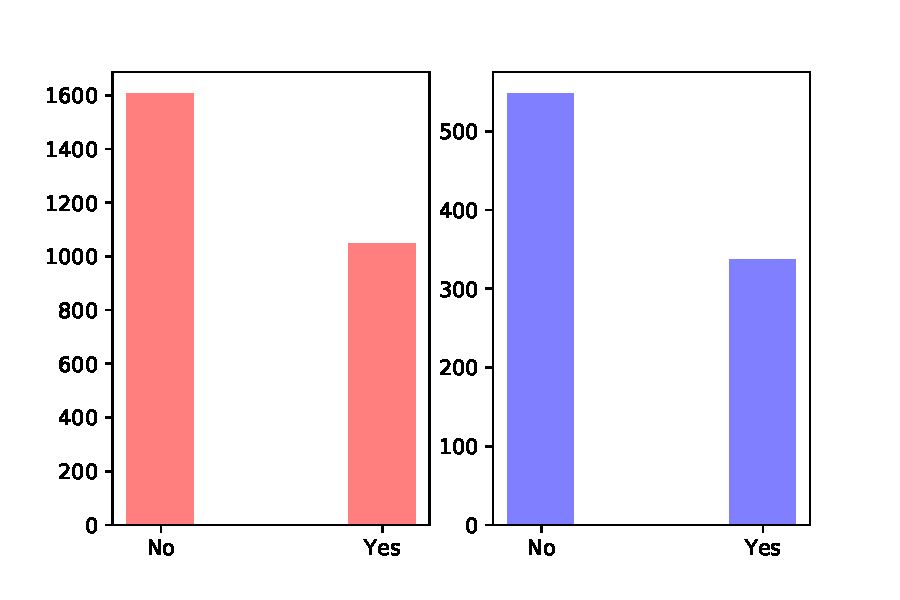
\includegraphics[width=1.1\columnwidth]{Figures/distribution.pdf}
    \caption{Distribution of relevance on train and test set}
    \label{fig:fig1}
\end{figure}

\subsubsection{Naive Bayes}
The simplest model that we tried was \textit{Naive Bayes} which assumes that words in the sentence are independent.
The results we obtained are shown in Table~\ref{tab:tab1}.

\begin{table}[h]
    \centering
    \begin{tabular}{ c | c c c c } 
         & Accuracy & Precision & Recall & F1 \\ 
         \hline
         Relevance & 0.84 & 0.79 & 0.79 & 0.79 \\
         Categories & 0.70 & / & / & 0.68 \\
    \end{tabular}
    \caption{Evaluation of Naive Bayes}
    \label{tab:tab1}
\end{table}

Although the model is naive, the results we got are not that bad.
The AUC of the model for predicting the relevance of the text is 91\%.

\subsubsection{Logistic Regression}
The results of Logistic Regression model are in Table~\ref{tab:tab2}.

\begin{table}[h]
    \centering
    \begin{tabular}{ c | c c c c } 
         & Accuracy & Precision & Recall & F1 \\ 
         \hline
         Relevance & 0.84 & 0.87 & 0.70 & 0.78 \\
         Categories & 0.74 & / & / & 0.72 \\
    \end{tabular}
    \caption{Evaluation of Logistic Regression}
    \label{tab:tab2}
\end{table}

The performance is similar to \textit{Naive Bayes}.
But we go the AUC of 93\% which is the highest of all baseline models.

\subsubsection{Support Vector Machine}
The results we got with this model are in Table~\ref{tab:tab3}.

\begin{table}[h]
    \centering
    \begin{tabular}{ c | c c c c } 
         & Accuracy & Precision & Recall & F1 \\ 
         \hline
        Relevance & 0.86 & 0.87 & 0.73 & 0.80 \\ 
        Categories & 0.74 & / & / & 0.73 \\
    \end{tabular}
    \caption{Evaluation of Support Vector Machine}
    \label{tab:tab3}
\end{table}

Overall SVM performed the best so we will use it in further experiments.
We also plotted the ROC curve for predicting the relevance of the text which is shown on Figure~\ref{fig:fig2}.

\begin{figure}[h]
    \centering
    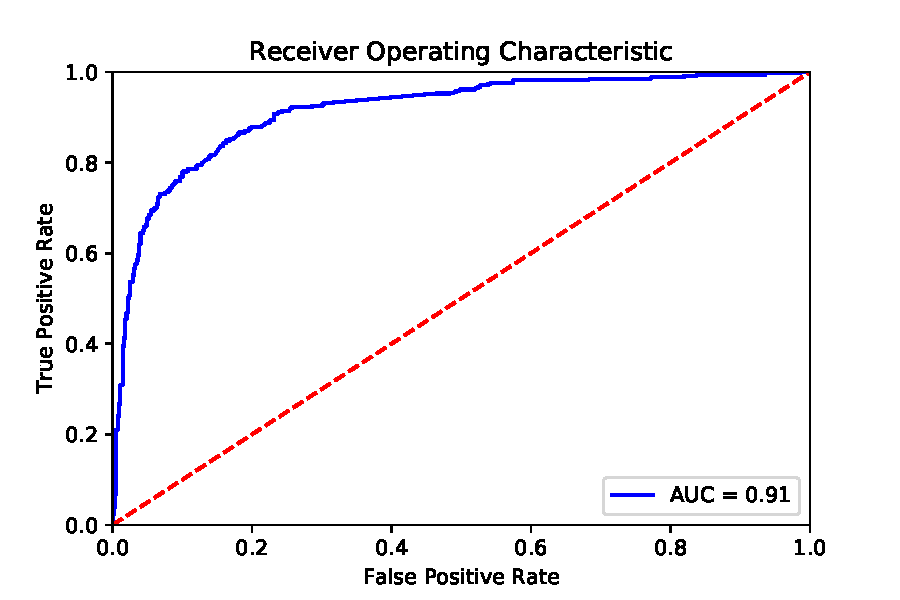
\includegraphics[width=1.0\columnwidth]{Figures/rocsvm.pdf}
    \caption{ROC curve of SVM performance}
    \label{fig:fig2}
\end{figure}

\subsection{Detecting of conversation drift}
To detect when the teacher needs to intervene we trained two models.
They were trained using the lemmatized texts as before.
But in this case we took sequential texts to train and test our models.
For training we took first 70\% of lemmatized texts and calculate their Tf-idf vectors.
From the experiments above we decided to train SVM model for classification of relevance of the text and Linear Regression (LR) for classification of category.
Both of the models were trained and evaluated using the 5-fold cross validation.
The accuracy and F1 score of SVM model were 0.83 and 0.82 respectively.
For the LR model we obtained 0.65 accuracy and 0.67 F1 score.

The last 30\% of conversations we used as to detect the drift.
We took the baches of 10 sequential messages and for each we predicted the relevance label.
We counted the number of relevance chats in a bach using the following method.
If the label was positive ('Yes') we counted it as relevant.
If the label was negative ('No') we also predicted the category.
We defined three soft categories ('C','S','M') which also count as relevant.
If the category was any of those we classified chat as relevant otherwise as non-relevant.
From the frequency of relevant/non-relevant chats we classified each bach.
The drift is detected if there is non relevant discussion in 5 consecutive baches.


% \iftaclpubformat
% \section{Courtesy warning: Common violations of \taclpaper rules that have
% resulted in papers being returned to authors for corrections}

% Avoid publication delays by avoiding these.
% \begin{enumerate}
% \item Violation: incorrect parentheses for in-text citations.  See \S
% \ref{sec:in-text-cite} and Table \ref{tab:cite-commands}.
% \item Violation: URLs that, when clicked, yield an error such as a 404 or go
% to the wrong page.
%   \begin{itemize}
%      \item Advice: best scholarly practice for referencing URLS would be to also
%      include the date last accessed.
%   \end{itemize}
% \item Violation: non-fulfillment of promise from submission to provide access
% instructions (such as a URL) for code or data.
% \item Violation: References incorrectly formatted (see \S\ref{sec:references}).
% Specifically:
% \begin{enumerate}
%   \item Violation: initials instead of full first/given names in references.
%   \item Violation: missing periods after middle initials.
%   \item Violation: incorrect capitalization.  For example, change ``lstm'' to
%   LSTM and ``glove'' to GloVe.
%   \begin{itemize}
%     \item Advice: if using BibTex, apply curly braces within the title field to
%     preserve intended capitalization.
%   \end{itemize}
%   \item Violation: using ``et al.'' in a reference instead of listing all
%   authors of a work.
%   \begin{itemize}
%     \item Advice: List all authors and check accents on author names even when
%     dozens of authors are involved.
%   \end{itemize}
%   \item Violation: not giving a complete arXiv citation number.
%   \begin{itemize}
%      \item Advice: best scholarly practice would be to give not only the full
%      arXiv number, but also the version number, even if one is citing version 1.
%   \end{itemize}
%   \item Violation: not citing an existing peer-reviewed version in addition to
%   or instead of a preprints
%     \begin{itemize}
%      \item Advice: When preparing the camera-ready, perform an additional check
%      of preprints cited to see whether a peer-reviewed version has appeared
%      in the meantime.
%   \end{itemize}
%   \item Violation: book titles do not have the first initial of all main words
%   capitalized.
%   \item Violation: In a title, not capitalizing the first letter of the first word
%   after a colon or similar punctuation mark.
% \end{enumerate}
% \end{enumerate}
% \else
% % Submission-specific rules
% \section{Courtesy warning: Common violations of \taclpaper rules that have
% resulted in desk
% rejects}
% \begin{enumerate}
%   \item Violation: wrong paper format.
%   \emph{As of the September 2018 submission round and beyond, TACL requires A4
%   format.  This is a change from the prior paper size.}

%   \item Violation: main document text smaller than 11pt, or table or figure
%   captions in a font smaller than 10pt. See Table \ref{tab:font-table}.

%   \item Violation: fewer than seven pages of content or more than ten pages of
%   content, {\em including} any appendices. (Exceptions are made for
%   re-submissions where a TACL Action Editor explicitly granted a set number of
%   extra pages to address reviewer comments.) See
%   Section \ref{sec:length}.
%   \item Violation: Author-identifying information in the document content or
%   embedded in the file itself.
%     \begin{itemize}
%       \item Advice: Make sure the submitted PDF does \emph{not} embed within it
%       any author info: check the document properties before submitting.
%       Useful tools include Adobe Reader and {\tt pdfinfo}.
%       \item Advice: Check that no URLs (or corresponding websites) inadvertently
%       disclose any author information. If software or data is to be distributed,
%       mention so in {\em anonymized} fashion.
%       \item Advice: Make sure that author names have been omitted
%       from the author block. (It's OK to include some sort of anonymous
%       placeholder.)
%       \item Advice: Do not include acknowledgments in a submission.
%       \item Advice: While citation of one's own relevant prior work is as
%       encouraged as the citation of any other relevant prior work,
%       self-citations should be made in the third, not first, person.
%       No citations should be attributed to ``anonymous'' or the like.
%       See Section \ref{sec:self-cite}.
%     \end{itemize}
% \end{enumerate}
% \fi


% \section{General instructions}

% \Taclpapers that do not comply with this document's instructions
% risk
% \iftaclpubformat
% publication delays until the camera-ready is brought into compliance.
% \else
% rejection without review.
% \fi


% \Taclpapers should consist of a Portable Document Format (PDF) file formatted
% for  \textbf{A4 paper}.\footnote{Prior to the September 2018 submission round, a
% different paper size was used.} All necessary fonts should be
% included in the  file.

% \iftaclpubformat
% Note that you will need to provide both a single-spaced and a double-spaced
% version; see \S \ref{ssec:layout}.

% If you promised to provide code or data at submission, specific instructions for
% how to access such resources must be provided.  (Typically, a URL to a stable,
% resource-specific site suffices.)

% All URLs should be manually checked to verify that they
% lead to a valid webpage, and to the site that was intended.
% \fi


% \section{\LaTeX\ files}

% \LaTeX\ files compliant with these instructions are available at the
% Author Guidelines section of the
% TACL website, \href{https://www.transacl.org/}
% {https://www.transacl.org}.\footnote{Last accessed \dateOfLastUpdate.} Use of the
% TACL \LaTeX\ files is highly recommended: \emph{MIT Press requires authors to
% supply \LaTeX\ source files as part of the publication process}; and
% use of the recommended \LaTeX\ files makes conversion to the
% required camera-ready format simple.
% \iftaclpubformat
% Specifically, the conversion can be accomplished by as little as: (1) add
% ``acceptedWithA'' in the square brackets in the line invoking the TACL package,
% like so:
% {\footnotesize {\tt {\textbackslash usepackage}[acceptedWithA]\{\styleFileVersion\}}} (2) add author information;
% (3) add acknowledgments.
% \fi

% \subsection{Workarounds for problems with the hyperref package}

% The provided files use the hyperref package by default. The TACL files
% employs the hyperref package to make clickable links for URLs and other references,
% and to make titles of bibliographic items into clickable links to their DOIs
% in the generated pdf.\footnote{Indeed, for some versions of acl\_natbib.sty,
% DOIs and URLs are not printed out or included in the bibliography in any form
% if the hyperref package is not used.}

% However, it is known that citations or URLs that cross pages can trigger the
% compilation error ``{\tt {\textbackslash}pdfendlink ended up in different nesting
% level than {\textbackslash}pdfstartlink}''.  In such cases, you may temporarily
% disable the hyperref package and then compile to locate the offending portion of
% the tex file; edit to avoid a pagebreak within a link;\footnote{If the problematic
% link is part of a reference in the bibliography and you do not wish to
% directly edit the corresponding .bbl file, a heavy-handed approach is to
% add the line
% {\tt \textbackslash interlinepenalty=10000}
% just after the line
% {\tt \textbackslash sloppy\textbackslash clubpenalty4000\textbackslash widowpenalty4000} in the
% ``{\tt \textbackslash def\textbackslash thebibliography}'' portion
% of the file \styleFileVersion.sty.  This penalty means that LaTex will not allow
% individual bibliography items to cross a page break.
% }
%  and then re-enable the
% hyperref package.

% To disable it,
% add {\tt nohyperref} in the square brackets to pass that option to the TACL package.
% For example, change
% \iftaclpubformat
% \verb+[acceptedWithA]+ in
% {\footnotesize {\tt {\textbackslash usepackage}[acceptedWithA]\{\styleFileVersion\}}}
% to
% \verb+[acceptedWithA,nohyperref]+.
% \else
% {\tt {\textbackslash usepackage}[]\{\styleFileVersion\}}
% to
% {\tt {\textbackslash usepackage}[nohyperref]\{\styleFileVersion\}}.
% \fi



% \section{Length limits}
% \label{sec:length}

% \iftaclpubformat
% Camera-ready documents may consist of as many pages of content as allowed by
% the Action Editor in their final acceptance letter.
% \else
% Submissions may consist of seven to ten (7-10) A4 format (not letter) pages of
% content.
% \fi

% The page limit \emph{includes} any appendices. However, references
% \iftaclpubformat
% and acknowledgments
% \fi
% do not count
% toward the page limit.

% \iftaclpubformat
% \else
% Exception: Revisions of (b) or (c) submissions may have been allowed
% additional pages of content by the prior Action Editor, as specified in their
% decision letter.
% \fi

% \section{Fonts and text size}

% Adobe's {Times Roman} font should be used. In \LaTeX2e{} this is accomplished by
% putting \verb+\usepackage{times,latexsym}+ in the preamble.\footnote{Should
% Times Roman be unavailable to you, use
% {Computer Modern Roman} (\LaTeX2e{}'s default).  Note that the latter is about
% 10\% less dense than Adobe's Times Roman font.}

% Font size requirements are listed in Table \ref{tab:font-table}. In addition to
% those requirements, the content of figures, tables, equations, etc. must be
% of reasonable size and readability.
% \begin{table}[t]
% \begin{center}
% \begin{tabular}{|l|rl|}
% \hline \bf Type of Text & \bf Size & \bf Style \\ \hline
% paper title & 15 pt & bold \\
% \iftaclpubformat
% author names & 12 pt & bold \\
% author affiliation & 12 pt & \\
% \else
% \fi
% the word ``Abstract'' as header & 12 pt & bold \\
% abstract text & 10 pt & \\
% section titles & 12 pt & bold \\
% document text & 11 pt  &\\
% captions & 10 pt & \\
% %bibliography & 10 pt & \\
% footnotes & 9 pt & \\
% \hline
% \end{tabular}
% \end{center}
% \caption{\label{tab:font-table} Font requirements}
% \end{table}




% \section{Page Layout}
% \label{ssec:layout}


% The margin dimensions for a page in A4 format (21 cm $\times$ 29.7 cm) are given
% in Table \ref{tab:margin-table}.  Start the content of all pages directly under
% the top margin.
% \iftaclpubformat
% \else
% (The confidentiality header (\S\ref{sec:ruler-and-header}) for submissions is an
% exception.)
% \fi


% \begin{table}[ht]
% \begin{center}
% \begin{tabular}{|l|}  \hline
% Left and right margins: 2.5 cm \\
% Top margin: 2.5 cm \\
% Bottom margin: 2.5 cm \\
% Column width: 7.7 cm \\
% Column height: 24.7 cm \\
% Gap between columns: 0.6 cm \\ \hline
% \end{tabular}
% \end{center}
% \caption{\label{tab:margin-table} Margin requirements}
% \end{table}


% \Taclpapers must be in two-column format.
% Allowed exceptions to the two-column format are the title, which must be
% centered at the top of the first page;
% \iftaclpubformat
% the author block containing author names and affiliations and addresses, which
% must be centered on the top of the first page and placed after the title;
% \else
% the  confidentiality header (see \S\ref{sec:ruler-and-header}) on submissions;
% \fi
% and any full-width figures or tables.

% Should the pages be numbered?  Yes, for submissions (to facilitate review); but
% no, for camera-readies (page numbers will be added at publication time).

% \Taclpapers should be single-spaced.
% \iftaclpubformat
% But, {\em an additional double-spaced version must also be provided, together with the
% single-spaced version, for the use of the copy-editors.}  A double-spaced version can
% be created by adding the ``copyedit'' option: Change \verb+[acceptedWithA]+ in
% {\footnotesize {\tt {\textbackslash usepackage}[acceptedWithA]\{\styleFileVersion\}}}
% to \verb+[acceptedWithA,copyedit]+.
% \fi

% {Indent} by about 0.4cm when starting a new paragraph that is not the first in a
% section or subsection.

% \subsection{The confidentiality header and line-number ruler}
% \label{sec:ruler-and-header}
% \iftaclpubformat
% Camera-readies should not include the left- and right-margin line-number rulers
% or headers from the submission version.
% \else
% Each page of the submission should have the header ``\confidentialtext''
% centered across both columns in the top margin.

% Submissions must include line numbers in the left and right
% margins, as demonstrated in the TACL submission-formatting
% instructions pdf file, because the line numbering allows reviewers to be very
% specific in their comments.\footnote{Authors using Word to prepare their
% submissions can create the marginal line numbers by inserting text
% boxes containing the line numbers.}
% Note that the numbers on the ruler need not line up exactly with the text lines
% of the paper. (Indeed, the line numbers generated by the recommended \LaTeX\
% files typically do not correspond exactly to the text lines.)
% \fi

% The presence or absence of the ruler or header should not change the appearance
% of any other content on the page.



% \begin{table*}[t]
% \centering
% \begin{tabular}{p{7.8cm}@{\hskip .5cm}p{7.8cm}}
% \multicolumn{1}{c}{{\bf Incorrect}} & \multicolumn{1}{c}{{\bf Correct}} \\  \hline
% ``\ex{(Cardie, 1992) employed learning.}'' &
% ``\ex{Cardie (1992) employed learning.}'' \\
% {The problem}:  ``employed learning.'' is not a sentence.  & Create by
% \verb+\citet{+\ldots\verb+}+  or \verb+\newcite{+\ldots\verb+}+. \\
% \\  \hline
% ``\ex{The method of (Cardie, 1992) works.}'' &
% ``\ex{The method of Cardie (1992) works.}''  \\
% {The problem}:  ``The method of was used.'' is not a sentence.  & Create as
% above.\\ \\\hline
% ``\ex{Use the method of (Cardie, 1992).}'' &
% ``\ex{Use the method of Cardie (1992).}''  \\
% {The problem}:  ``Use the method of.'' is not a sentence.  & Create as
% above.\\ \\\hline
% \ex{Related work exists Lee (1997).} & \ex{Related work exists (Lee,
% 1997).} \\
% {The problem}:  ``Related work exists Lee.'' is not a sentence (unless one
% is scolding a Lee). & Create by
% \verb+\citep{+\ldots\verb+}+  or \verb+\cite{+\ldots\verb+}+. \\
% \\  \hline
% \end{tabular}
% \caption{\label{tab:cite-commands} Examples of incorrect and correct citation
%   format.  Also depicted are citation commands supported by the
%   tacl2018.sty file, which is based on the natbib package and
%   supports all natbib citation commands.
%   The tacl2018.sty file also supports commands defined in previous ACL style
%   files
%   for compatibility.
%   }
% \end{table*}





% \section{The First Page}
% \label{ssec:first}

% Center the title, which should be placed 2.5cm from the top of the page,
% \iftaclpubformat
% and author names and affiliations
% \fi
% across both columns of the first page. Long titles should be typed on two lines
% without a blank line intervening.
% \iftaclpubformat
% After the title, include a blank line before the author block.
% Do not use only initials for given names, although middle initials are allowed.
% Do not put surnames in all capitals.\footnote{Correct: ``Lillian Lee'';
% incorrect: ``Lillian LEE''.} Affiliations should include authors' email
% addresses. Do not use footnotes for affiliations.
% \else
% Do not include the paper ID number assigned during the submission process.
% \fi

% \iftaclpubformat
% \else
% Although submissions should not include any author information, maintain space
% for names and affiliations/addresses so that they will fit in the final
% (camera-ready)
% version.
% \fi


% Start the abstract at the beginning of the first
% column, about 8 cm from the top of the page, with the centered header
% ``Abstract'' as specified in Table \ref{tab:font-table}.
% The width of the abstract text
% should be narrower than the width of the columns for the text in the body of the
% paper by about 0.6cm on each side.

% \section{Section headings}

% Use numbered section headings (Arabic numerals) in order to facilitate cross
% references. Number subsections with the section number and the subsection number
% separated by a dot.



% \section{Figures and Tables}

% Place figures and tables in the paper near where they are first discussed.

% Provide a caption for every illustration. Number each one
% sequentially in the form:  ``Figure 1: Caption of the Figure.'' or ``Table 1:
% Caption of the Table.''

% Authors should ensure that tables and figures do not rely solely on color to
% convey critical distinctions and are, in general,  accessible to the
% color-blind.



% \section{Citations and references}
% \label{sec:cite}


% \subsection{In-text citations}
% \label{sec:in-text-cite}
% Use correctly parenthesized author-date citations
% (not numbers) in the text. To understand correct parenthesization, obey the
% principle that \emph{a sentence containing parenthetical items should remain
% grammatical when the parenthesized material is omitted.} Consult Table
% \ref{tab:cite-commands} for usage examples.


% \iftaclpubformat
% \else
% \subsection{Self-citations}
% \label{sec:self-cite}

% Citing one's own relevant prior work should be done,  but use the third
% person instead of the first person, to preserve anonymity:
% \begin{tabular}{l}
% Correct: \ex{Zhang (2000) showed ...} \\
% Correct: \ex{It has been shown (Zhang, 2000)...} \\
% Incorrect: \ex{We (Zhang, 2000) showed ...} \\
% Incorrect: \ex{We (Anonymous, 2000) showed ...}
% \end{tabular}
% \fi

% \subsection{References}
% \label{sec:references}
% Gather the full set of references together under
% the boldface heading ``References''. Arrange the references alphabetically
% by first author's last/family name, rather than by order of occurrence in the
% text.

% References to peer-reviewed publications should be given in addition to or
% instead of preprint versions. When giving a reference to a preprint, including
% arXiv preprints, include the number.

% List all authors of a given reference, even if there are dozens; do not
% truncate the author list with an ``et al.''  Use full first/given names for
% authors, not initials.  Include periods after middle initials.

% Titles should have correct capitalization.  For example, change change
% ``lstm'' or ``Lstm'' to ``LSTM''.\footnote{If using BibTex, apply curly braces
% within the title field to preserve intended capitalization.}   Capitalize the
% first letter of the first word after a colon or similar punctuation mark.  For
% book titles, capitalize the first letter of all main words.  See the
% reference entry for \citet{Jurafsky+Martin:2009a} for an example.


% We strongly encourage the following, but do not absolutely mandate them:
% \begin{itemize}
% \item Include DOIs.\footnote{The supplied \LaTeX\ files will
% automatically add hyperlinks to the DOI when BibTeX or
% BibLateX are invoked if the hyperref package is used and
% the doi field is employed in the corresponding bib entries.
% The DOI itself will not be separately printed out in that case.}
% \item Include the version number when citing arXiv preprints, even if only one
% version exists at the time of writing.
% For example,\footnote{Bibtex entries for \citet{DBLP:journals/corr/cs-CL-0108005} and
% \citet{DBLP:journals/corr/cs-CL-9905001} corresponding to the depicted output
% can be found in the supplied sample file {\tt tacl.bib}.  We also cite
% the peer-reviewed versions \cite{GOODMAN2001403,P99-1010}, as required.}
% note the ``v1'' in the following.
% \begin{quote}
% Joshua Goodman.  2001.  A bit of progress in language modeling. {\it CoRR},
% cs.CL/0108005v1.
% \end{quote}
% An alternative format is:
% \begin{quote}
% Rebecca Hwa. 1999. Supervised grammar induction using training data with limited constituent
% information. {cs.CL/9905001}. Version 1.
% \end{quote}
% \end{itemize}

% \section{Appendices} Appendices, if any, directly follow the text and the
% references.  Recall from Section \ref{sec:length} that {\em appendices count
% towards the page
% limit.}


% \iftaclpubformat

% \section{Including acknowledgments}
% Acknowledgments appear immediately before the references.  Do not number this
% section.\footnote{In \LaTeX, one can use {\tt {\textbackslash}section*} instead
% of {\tt {\textbackslash}section}.} If you found the reviewers' or Action
% Editor's comments helpful, consider acknowledging them.
% \else
% \fi

% \section{Contributors to this document}
% \label{sec:contributors}

% This document was adapted by Lillian Lee and Kristina Toutanova
% from the instructions and files for ACL 2018, by Shay Cohen, Kevin Gimpel, and
% Wei Lu. Those files were drawn from earlier *ACL proceedings, including those
% for ACL 2017 by Dan Gildea and Min-Yen Kan, NAACL 2017 by Margaret Mitchell,
% ACL 2012 by Maggie Li and Michael White, those from ACL 2010 by Jing-Shing
% Chang and Philipp Koehn, those for ACL 2008 by Johanna D. Moore, Simone
% Teufel, James Allan, and Sadaoki Furui, those for ACL 2005 by Hwee Tou Ng and
% Kemal Oflazer, those for ACL 2002 by Eugene Charniak and Dekang Lin, and
% earlier ACL and EACL formats,  which were written by several people,
% including John Chen, Henry S. Thompson and Donald Walker. Additional elements
% were taken from the formatting instructions of the {\em International Joint
% Conference on Artificial   Intelligence} and the \emph{Conference on Computer
% Vision and Pattern Recognition}.

% \bibliographystyle{IEEEtran}
\bibliographystyle{acl_natbib}
\bibliography{bibliography}

\end{document}


